\documentclass[border=3pt]{standalone}
% Preâmbulo compartilhado pelos diagramas TikZ da aula 9 de IHC (Princípios e Diretrizes)
\usepackage[T1]{fontenc}
\usepackage[utf8]{inputenc}
\usepackage{lmodern}
\usepackage{amsmath}
\usepackage{xcolor}
\usepackage{tikz}
\usetikzlibrary{arrows.meta,angles,quotes,decorations.pathmorphing,decorations.pathreplacing,calc,
                positioning,shapes.geometric,shapes.misc,backgrounds,fit,
                math}

% Paleta (mesma dos SVGs originais)
% Paleta da disciplina de IHC: acento roxo (#755099), da capa do livro.
% (o nome "dblue" é mantido para não alterar todos os diagramas)
\definecolor{dblue}{HTML}{755099}
\definecolor{dorange}{HTML}{B3541E}
\definecolor{dgreen}{HTML}{4A7C59}
\definecolor{dred}{HTML}{9C4B4B}
\definecolor{dcream}{HTML}{F4F1EA}
\definecolor{dshade}{HTML}{DDD7C9}

% Função gaussiana (não normalizada por padrão de escala visual)
\pgfmathdeclarefunction{gauss}{3}{%
  \pgfmathparse{1/(#3*sqrt(2*pi))*exp(-((#1-#2)^2)/(2*#3^2))}%
}

% Estilos comuns (prefixo d... para não colidir com chaves internas do pgf)
\tikzset{
  >={Stealth[length=2mm]},
  dguide/.style={gray!55, dashed, line width=0.4pt},
  daxis/.style={gray!60, line width=0.7pt, ->},
  dbody/.style={fill=black!3, draw=black!80, line width=1pt},
  dacc/.style={draw=dblue, line width=1pt},
  dlbl/.style={black!55, font=\small},
  dsub/.style={black!45, font=\footnotesize},
  dstate/.style={circle, draw=black!80, fill=dcream, line width=1pt,
                 minimum size=17mm, font=\large, inner sep=1pt},
  dobs/.style={circle, draw=black!80, fill=dshade, line width=1pt,
               minimum size=14mm, font=\large, inner sep=1pt},
  dbox/.style={rounded corners=2pt, draw=black!80, fill=dcream, line width=1pt,
               align=center, inner sep=6pt},
  dop/.style={circle, draw=black!80, fill=white, line width=1pt,
              minimum size=6mm, inner sep=0pt, font=\small},
  dtrans/.style={->, dblue, line width=1pt},
  dmeas/.style={->, dorange, line width=1pt},
  dcurve/.style={line width=1pt, dblue},
  dcurveb/.style={line width=1.4pt, dorange},
}

\begin{document}
\hyphenpenalty=10000 \exhyphenpenalty=10000 \tolerance=9999 \emergencystretch=3em
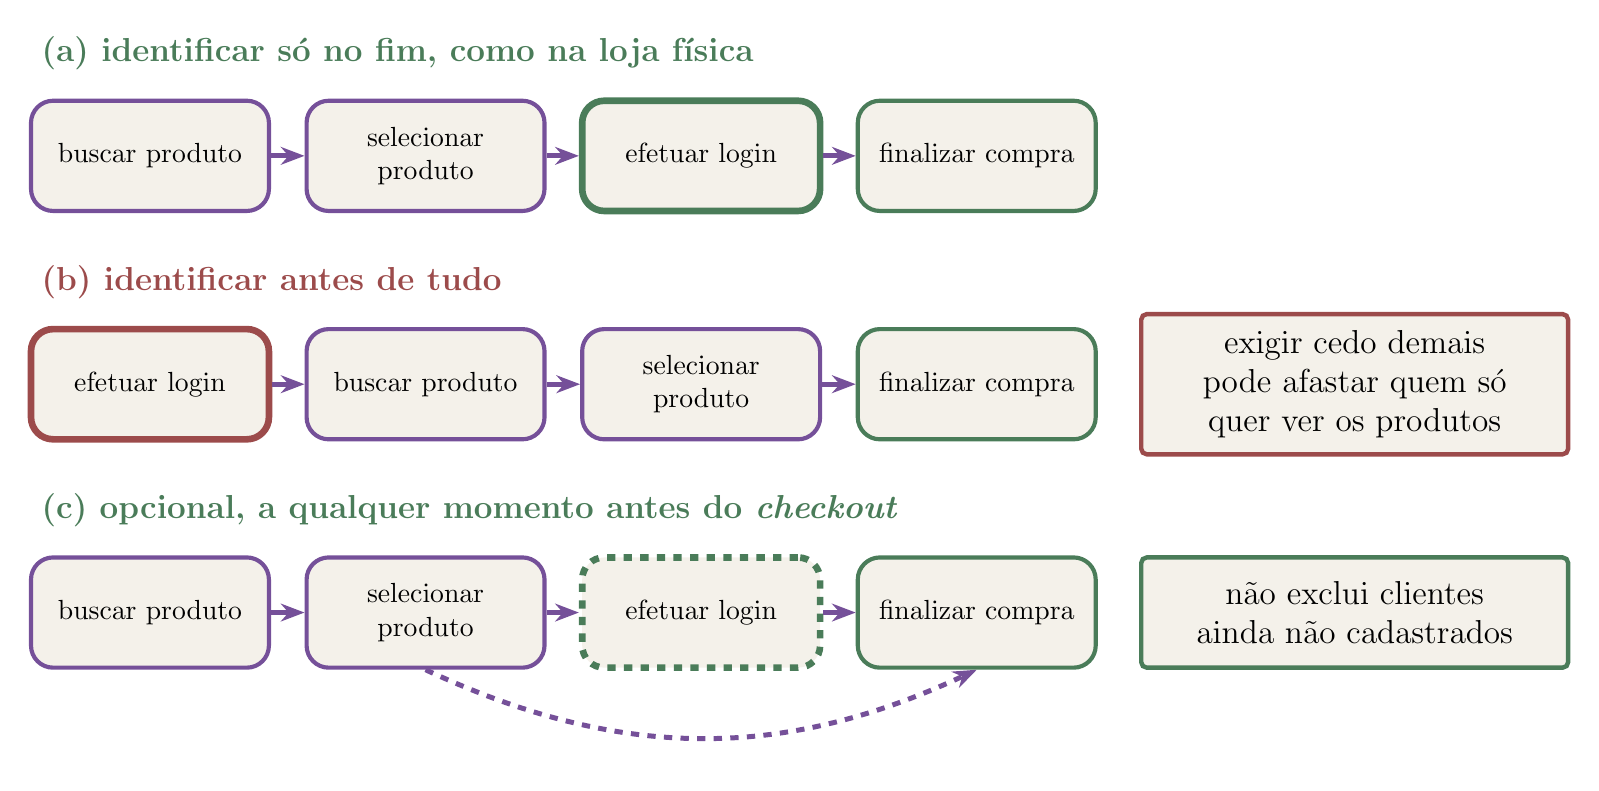
\begin{tikzpicture}[x=1cm,y=1cm]
\tikzset{s/.style={dbox, text width=2.6cm, minimum height=1.4cm, font=\normalsize, line width=1.5pt, rounded corners=8pt},
        a/.style={dtrans, line width=1.8pt, -{Stealth[length=3mm]}}}
\node[font=\large\bfseries, dgreen, anchor=west] at (0,8.6) {(a) identificar só no fim, como na loja física};
\node[s, draw=dblue] (a1) at (1.5,7.3) {buscar produto};
\node[s, draw=dblue] (a2) at (5.0,7.3) {selecionar produto};
\node[s, draw=dgreen, line width=2.4pt] (a3) at (8.5,7.3) {efetuar login};
\node[s, draw=dgreen] (a4) at (12.0,7.3) {finalizar compra};
\draw[a] (a1) -- (a2); \draw[a] (a2) -- (a3); \draw[a] (a3) -- (a4);
\node[font=\large\bfseries, dred, anchor=west] at (0,5.7) {(b) identificar antes de tudo};
\node[s, draw=dred, line width=2.4pt] (b1) at (1.5,4.4) {efetuar login};
\node[s, draw=dblue] (b2) at (5.0,4.4) {buscar produto};
\node[s, draw=dblue] (b3) at (8.5,4.4) {selecionar produto};
\node[s, draw=dgreen] (b4) at (12.0,4.4) {finalizar compra};
\draw[a] (b1) -- (b2); \draw[a] (b2) -- (b3); \draw[a] (b3) -- (b4);
\node[font=\large\bfseries, dgreen, anchor=west] at (0,2.8) {(c) opcional, a qualquer momento antes do \emph{checkout}};
\node[s, draw=dblue] (c1) at (1.5,1.5) {buscar produto};
\node[s, draw=dblue] (c2) at (5.0,1.5) {selecionar produto};
\node[s, draw=dgreen] (c4) at (12.0,1.5) {finalizar compra};
\node[s, draw=dgreen, dashed, line width=2.4pt] (c3) at (8.5,1.5) {efetuar login};
\draw[a] (c1) -- (c2); \draw[a] (c2) -- (c3); \draw[a] (c3) -- (c4);
\draw[a, dashed] (c2.south) to[bend right=25] (c4.south);
\node[dbox, draw=dgreen, text width=5.0cm, minimum height=1.4cm, font=\large, line width=1.6pt] at (16.8,1.5) {não exclui clientes ainda não cadastrados};
\node[dbox, draw=dred, text width=5.0cm, minimum height=1.4cm, font=\large, line width=1.6pt] at (16.8,4.4) {exigir cedo demais pode afastar quem só quer ver os produtos};
\end{tikzpicture}
\end{document}
